%\begin{figure}[t]
%	\centering
%	\includegraphics[width=0.7\columnwidth]{figures/ospfSynthesisTimeMCMC.eps}
%	\compactcaption{MCMC OSPF Synthesis time}
%	\label{fig:ospfmcmc}
%\end{figure}
\begin{figure*}
	\centering
	\subfloat[Synthesis Time]
	{\includegraphics[width=0.66\columnwidth]{figures/ospfTime.eps}}
	\subfloat[Number of Route Filters]
	{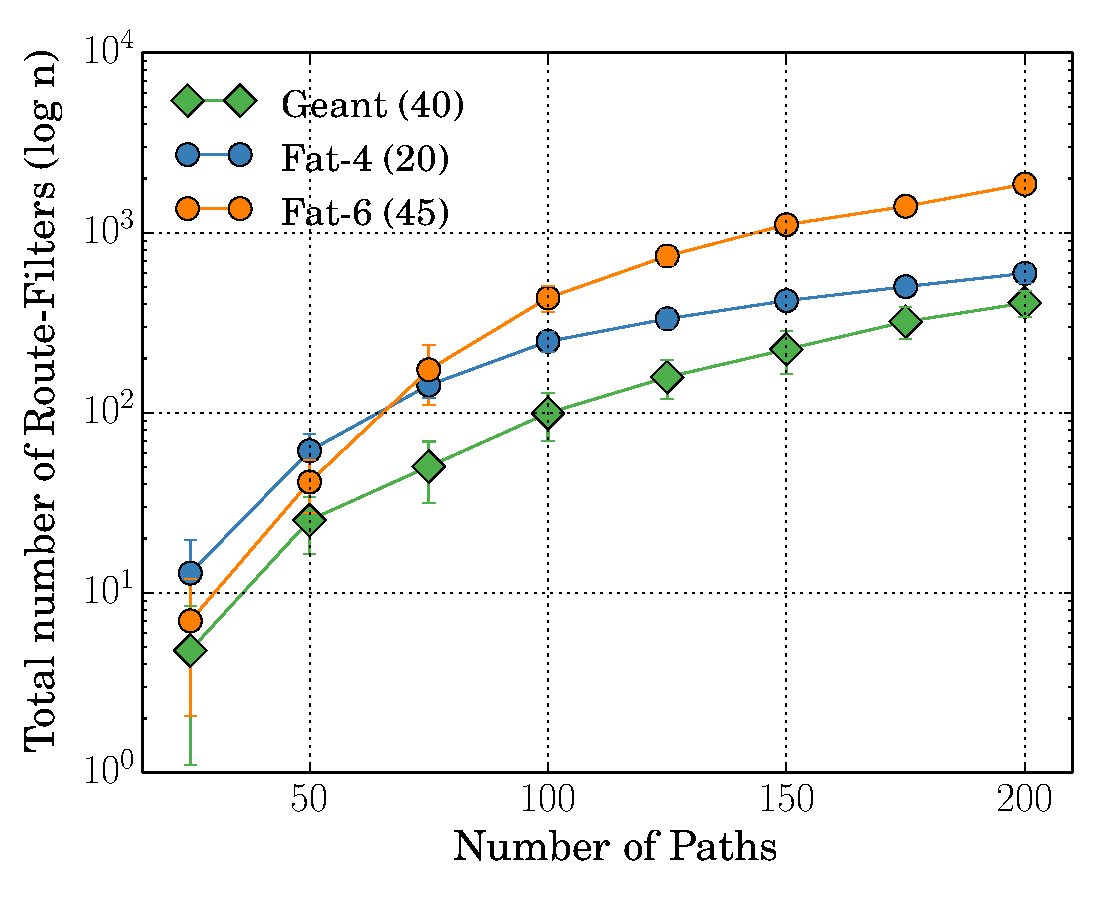
\includegraphics[width=0.66\columnwidth]{figures/ospfRF.eps}}
	\subfloat[Endpoint Resilience]
	{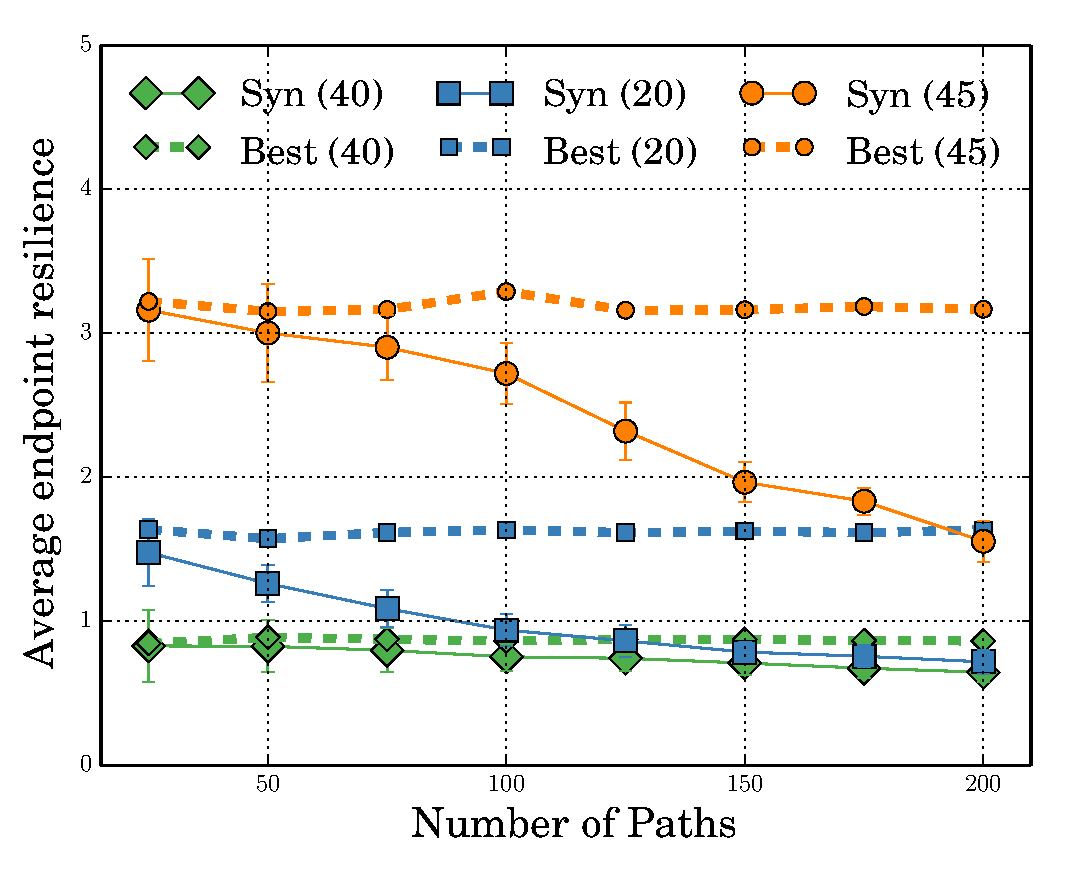
\includegraphics[width=0.66\columnwidth]{figures/ospfAvgRes.eps}}
	\compactcaption{\label{fig:ospfeval}
		OSPF Synthesis evaluation}
\end{figure*}


\begin{figure}
	\centering
	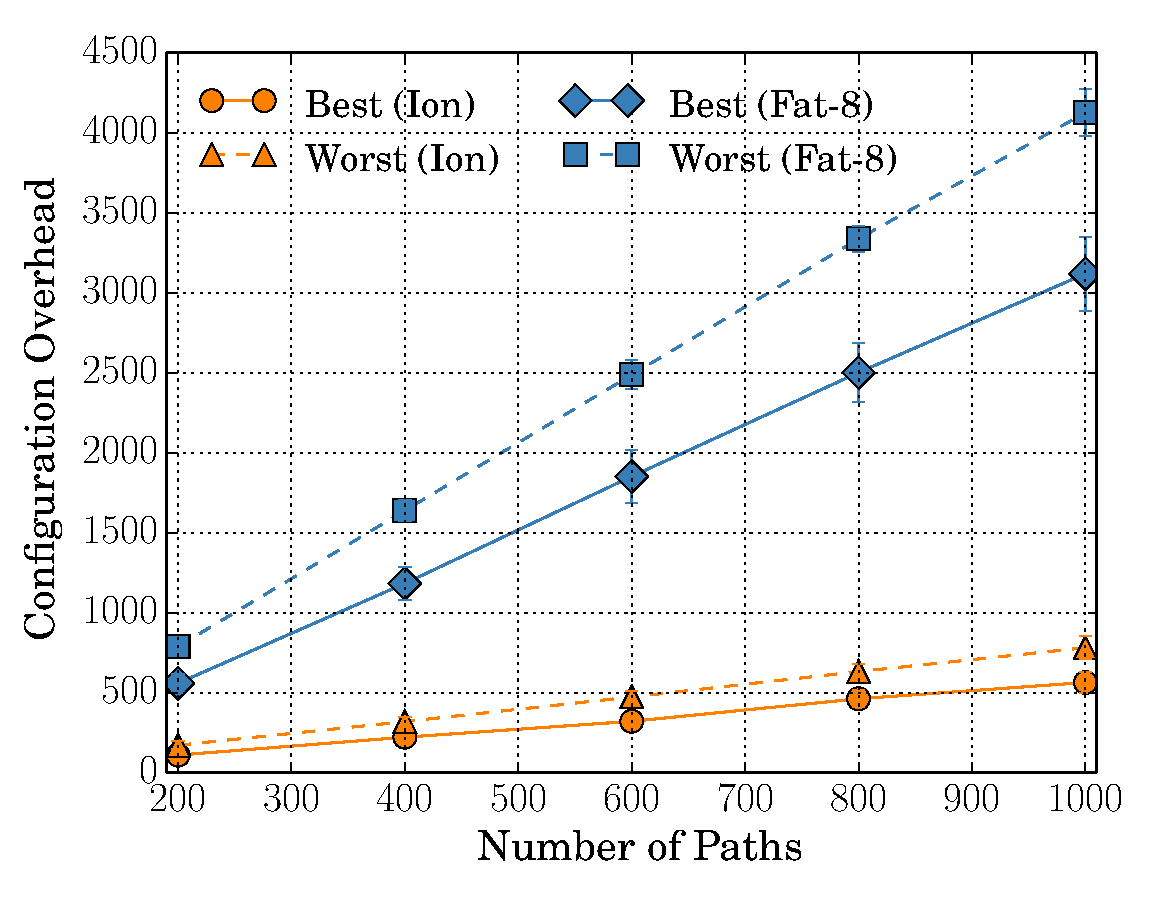
\includegraphics[width=0.7\columnwidth]{figures/confMCMC.eps}
	\compactcaption{MCMC Lines of Conf}
	\label{fig:confmcmc}
\end{figure}

\begin{figure}
	\centering
	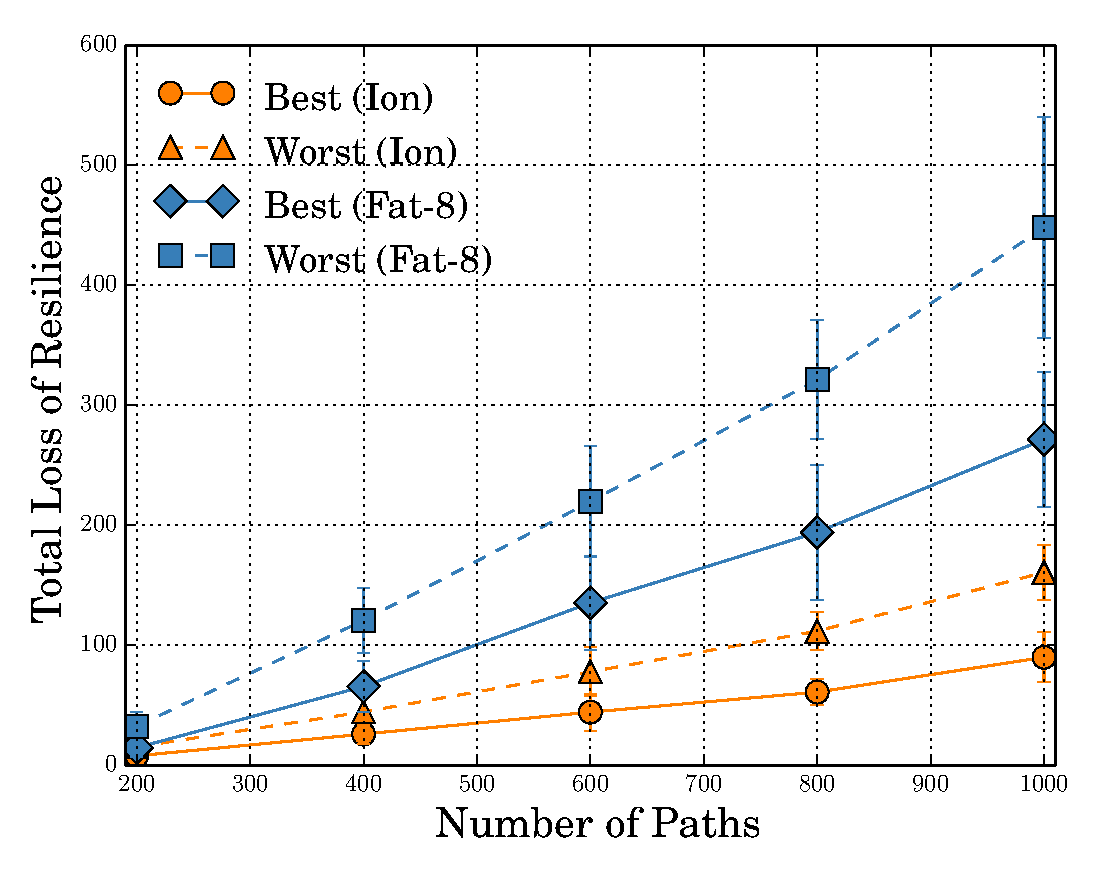
\includegraphics[width=0.7\columnwidth]{figures/TRLMCMC.eps}
	\compactcaption{MCMC TRL}
	\label{fig:trlmcmc}
\end{figure}

\begin{figure}
	\centering
	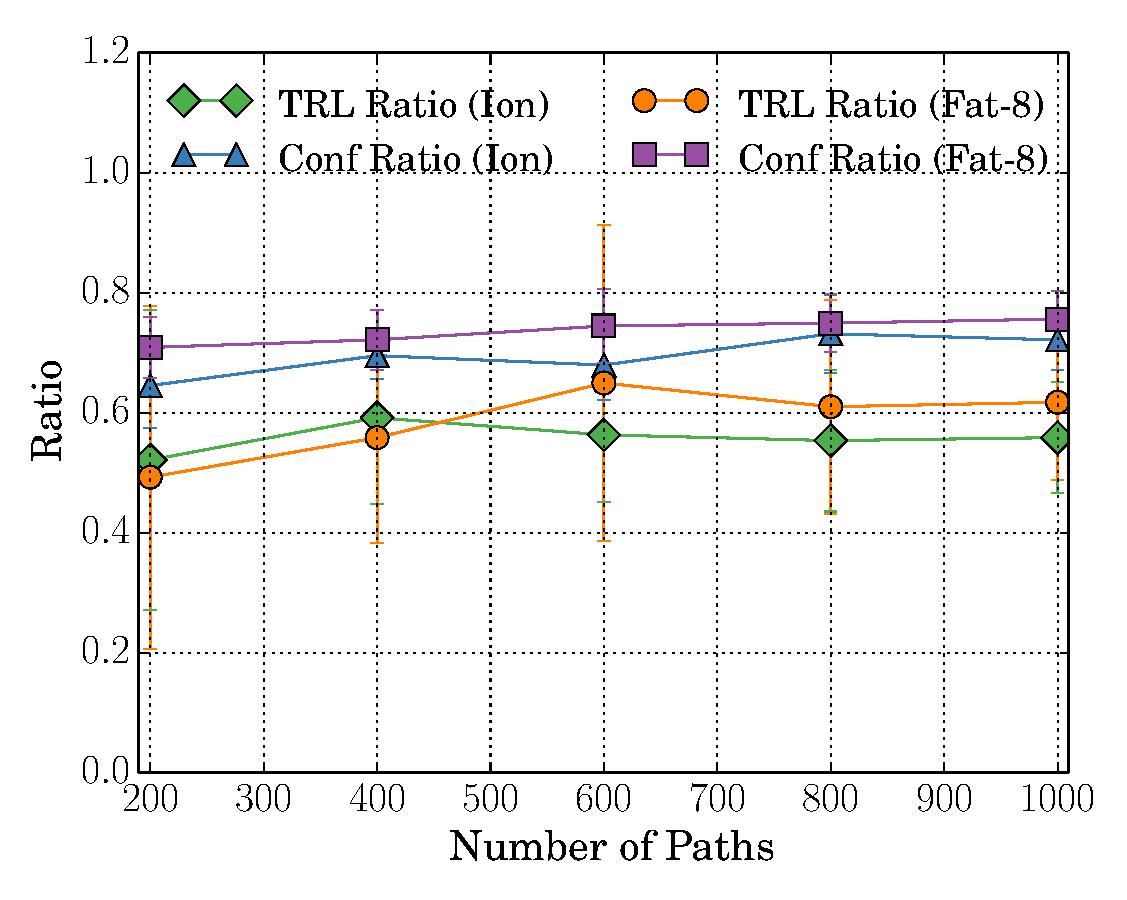
\includegraphics[width=0.7\columnwidth]{figures/ratioMCMC.eps}
	\compactcaption{MCMC Ratios}
	\label{fig:ratiomcmc}
\end{figure}




\section{Evaluation}
 \label{sec:evaluation}
 
 We implemented a full working
 prototype of \name in Python, which works as a standalone
 system or can be integrated with \genesis. For a given
 workload, \name outputs abstract configurations, which
 specifies the assignment of domains to different routers,
 the static routes, BGP configuration variables (local 
 preferences and iBGP filters), and the OSPF link weights
 and route-filters for each domain, which can be 
 translated to actual device configurations using templates~\cite{template}.
 \name uses the Gurobi LP solver~\cite{gurobi} for synthesis of 
 OSPF weights and filters. 
 
In this section, we evaluate \Name using
%\loris{really don't like the word realistic}
enterprise-scale multi-tenant data
center settings. 
Specifically, we ask:
\begin{compactitemize}
	\item What is the performance of \Name's baseline synthesis
	algorithm for tenant policies? How does the performance vary with size of the
	network, number and the nature of policies in use? (\secref{sec:baselineeval})
	
	\item What is the performance of \name for operator policies
	like capacity bounds, traffic engineering, and network repair
	which use SMT with linear optimization objectives and MaxSMT? (\secref{sec:optimizationeval})
	
	\item How much do tactics help improve \Name's 
	performance? Which tactics offer the best improvement? (\secref{sec:tacticeval})
	
	\item To what extent does the divide-and-conquer synthesis improve \Name's
	performance? When does it lead to degraded synthesis times? (\secref{sec:optimisticeval})
	
\end{compactitemize}


Ion (125 nodes) and Geant(40)

